%\RequirePackage{lineno}
%\documentclass[aps, prc, reprint, amsmath, groupedaddress, nofootinbib]{revtex4-1}
\documentclass[onecolumn,aps,superscriptaddress,nofootinbib,floatfix]{revtex4}
\usepackage{float}
\usepackage{listings}
\usepackage[utf8]{inputenc}
\usepackage{hyperref}
\usepackage{amsmath}
\usepackage{amssymb}
\usepackage{amsfonts}
\usepackage{tabularx}
\usepackage{booktabs}
\usepackage{graphicx}
\usepackage{subfigure}
\usepackage{color}
%\usepackage[switch]{lineno}
\usepackage{diagbox}
\usepackage{multirow}
\usepackage{bm}
\usepackage[inline]{enumitem}
\usepackage{algorithm} 
\usepackage{algpseudocode} 
%\usepackage{setspace}
\usepackage[T2A,T1]{fontenc}
\usepackage{mathrsfs}
\usepackage{amsmath}
\usepackage{amssymb}

\lstset{language=[LaTeX]TeX,keywordstyle=\color{red},showspaces=true,breaklines=true,breakatwhitespace=true,basicstyle=\small\tt,commentstyle=\color{white},frame=single,framerule=0pt,backgroundcolor=\color{yellow}}
\graphicspath{{fig/}}
\definecolor{theblue}{RGB}{0,50,230}

\usepackage{hyperref}
\hypersetup{
	colorlinks=true,
	linkcolor=theblue,
	citecolor=theblue,
	urlcolor=theblue
}
\newcommand{\pT} {\ensuremath{p_{\mathrm{T}}}}
\def\simge{\stackrel{>}{\sim} }
\def\simle{\stackrel{<}{\sim} }
\newcommand{\nch}{N_\text{ch}}
\newcommand{\sqrts}{\sqrt{s_{NN}}}
\newcommand{\T}{\tilde{T}}
\newcommand{\paddedhline}{\noalign{\smallskip}\hline\noalign{\smallskip}}
\newcommand {\avg}[1]{\ensuremath{\langle\kern-1.0pt\langle#1\rangle\kern-1.0pt\rangle}}
\newcommand{\dnchdy}{dN_\text{ch}/d\eta}
\newcommand{\dndypP}{dN_\text{pPb}/d\eta}
\newcommand{\dndyPP}{dN_\text{PbPb}/d\eta}
\newcommand{\dphi}    {\ensuremath{\Delta\phi}}
\newcommand{\x}{\mathbf x}
\newcommand{\y}{\mathbf y}
\newcommand{\z}{\mathbf z}
\newcommand{\trans}{^\intercal}
\newcommand{\La}{\langle}
\newcommand{\Ra}{\rangle}
\newcommand{\pttrg}      {\ensuremath{\pt^{a}}\xspace}
\newcommand{\ptass}      {\ensuremath{\pt^{b}}\xspace}
\newcommand{\avgevvn}[1]{\left\langle{#1}\right\rangle}
\newcommand{\Qf}[2]{\frac{\tilde{Q}_{#1}^{#2}}{|\tilde{Q}_{#1}^{#2}|}}
\newcommand{\Qfs}[2]{\frac{\tilde{Q}_{#1}^{*#2}}{|\tilde{Q}_{#1}^{#2}|}}
\newcommand{\lr}[1]{\left\langle #1\right\rangle}
\def\eq{{\,=\,}}
\newcommand{\avgev}[1]{\left\langle{#1}\right\rangle}
\def\bra{\langle}
\def\ket{\rangle}
\newlength\cmsFigWidth
\def\tq{T_q}
\def\ts{T_s}
\def\pt{p_T}
\def\bq{\begin{eqnarray}}
	\def\eq{\end{eqnarray}}

%%%%%%%%%%%%%%%%%%%%%%%%%%%%%%%%%%%%%%%%%%%%%%%%%%%%%%
\usepackage[normalem]{ulem}  % \sout{old text} for strikeout
%\usepackage[dvips]{color} % For blue in-text com ments and additions
\newcommand{\com}[1]{{\sf\color[rgb]{0,0,1}{#1}}}
\newcommand{\modi}[1]{{\sf\color[rgb]{1,0,0}{#1}}}
\newcommand{\ans}[1]{{\sf\color[rgb]{0,1,0}{#1}}}
\renewcommand\sout{\bgroup \color{red} \ULdepth=-.5ex \ULset}
%%%%%%%%%%%%%%%%%%%%%%%%%%%%%%%%%%%%%%%%%%%%%%%%%%%%%

\newcommand{\blue}[1]{{\color{blue}{#1}}}
\newcommand{\green}[1]{{\color{green}{#1}}}
\newcommand{\red}[1]{{\color{red}{#1}}}


\begin{document}
	%\linenumbers
	%%%%%%%%%%%%%%%%%%%%% Title %%%%%%%%%%%%%%%%%%%%%%
	
	\title{Formulae of Charmed Meson in Recombination Model}
	
	%%%%%%%%%%%%%%%%%%%% Authors %%%%%%%%%%%%%%%%%%%%%
	\author{Huanjing Gong}\email{gonghuanjing@stu.scu.edu.cn}
	\date{\today}
	
	%%%%%%%%%%%%%%%%%%%% Abstract %%%%%%%%%%%%%%%%%%%%%
	
	\pacs{}
	\keywords{}
	\maketitle
%	\tableofcontents

	Utility:
	\begin{eqnarray}
		\mathcal{S}^q(p)&=&\int{dq\over q} \sum_{i} F_i(q) QuenchF(q) S_i^q(p/q)QuenchS(p), \quad \text{if q=c, then i=charm, gluon}.\\
		\mathcal{SS}^{q_1 q_2}(p_1,p_2)&=&\int{dq\over q}  \sum_{i} F_i(q) QuenchF(q) S_i^{q_1}(p_1/q)QuenchS(p_1) S_i^{q_2}({p_2 \over q-p_1})QuenchS(p_2), \\
		&& \text{if q=c, then i=charm, gluon}.\nonumber \\
		R_M(p_1,p_2,p)&=&{g_M \over B(a+1,b+1)}({p_1 \over p})^{a+1} ({p_2 \over p})^{b+1} \delta({p_1 \over p}+{p_1 \over p}-1),\quad \text{in which }{a+1 \over b+1}\approx {m_1 \over m_2}. \\
		&& \text{for $D^0$, ${a+1 \over b+1}={1\over 5}$, for $D_s$, ${a+1 \over b+1}={3\over 10}$}.\nonumber \\
		xD_i^M(x)&=&\int_0^x {dx_1 \over x_1}\int_0^x {dx_2 \over x_2} \{S_i^q(x_1),S_i^{\overline{q'}} (x_2)\}R_M(x_1,x_2,x),\\
		QuenchF(q)&=&{1 \over 1+e^{(3.5-q)/0.5}},\\
		QuenchS(q)&=&1-e^{-(q/0.5)^2},\\
		QuenchD(q)&=&1-e^{-q^2}.
	\end{eqnarray}
	$J/\psi$:
	\begin{eqnarray}
		\frac{dN^{TT}_{J/\psi}}{p_Tdp_T}&=&{g_{J/\psi}C_c^2 p_T \over 4m_T^{J/\psi}}e^{-p_T/T_c}, \\
		\frac{dN^{TS}_{J/\psi}}{p_Tdp_T}&=&{g_{J/\psi}C_c \over 2m_T^{J/\psi}}e^{-p_T/2T_c}\mathcal{S}^c(p_T/2),\\
		\frac{dN^{SS^{1j}}_{J/\psi}}{p_Tdp_T}&=&{g_{J/\psi} \over p_T m_T^{J/\psi}}\mathcal{SS}^{c \bar{c}}(p_T/2,p_T/2),\\
		\frac{dN^{SS^{2j}}_{J/\psi}}{p_Tdp_T}&=&{g_{J/\psi}\Gamma \over p_T m_T^{J/\psi}}\mathcal{S}^c(p_T/2)\mathcal{S}^{\bar{c}}(p_T/2).
	\end{eqnarray}
	$D^0$:
	\begin{eqnarray}
		\frac{dN^{TT}_{D^0}}{p_Tdp_T}&=&{5g_{D^0} C_q C_c\over p_0 p_T^6}\int_0^{p_T}dp_1 p_1 e^{-p_1/T_q} (p_T -p_1) e^{-(p_T -p_1)/T_c} (p_T -p_1)^4, \\
		\frac{dN^{TS}_{D^0}}{p_Tdp_T}&=&{5g_{D^0} \over p_0 p_T^6}\int_0^{p_T}dp_1 
		p_1(p_T -p_1)^4 [C_q e^{-p_1/T_q} S^c(p_T-p_1)+C_c({p_T\over p_1} -1) e^{-(p_T -p_1)/T_c}S^{\bar{u}}(p_1)] , \\
		\frac{dN^{SS^{1j}}_{D^0}}{p_Tdp_T}&=&{1\over m_T^{D^0}}\int {dq \over q^2}\sum_{i=g,c} F_i(q)QuenchF(q)D_i^{D^0}(p_T/q)QuenchD(p_T), \\
		\frac{dN^{SS^{2j}}_{D^0}}{p_Tdp_T}&=&{5g_{D^0}\Gamma \over m_T^{D^0}p_T^6}\int_{0}^{p_T}dp_1 (p_T-p_1)^4 \mathcal{S}^{\bar{u}}(p_1) \mathcal{S}^{c}(p_T-p_1).
	\end{eqnarray}
	$D_s$:
	\begin{eqnarray}
		\frac{dN^{TT}_{D_s}}{p_Tdp_T}&=&{660g_{D_s} C_s C_c\over p_0 p_T^{13}}\int_0^{p_T}dp_1 p_1 e^{-p_1/T_s} (p_T -p_1) e^{-(p_T -p_1)/T_c} p_1^2 (p_T -p_1)^9, \\
		\frac{dN^{TS}_{D_s}}{p_Tdp_T}&=&{660g_{D_s} \over p_0 p_T^{13}}\int_0^{p_T}dp_1 
		p_1^3(p_T -p_1)^9 [C_s e^{-p_1/T_s} S^c(p_T-p_1)+C_c({p_T\over p_1} -1) e^{-(p_T -p_1)/T_c}S^{\bar{s}}(p_1)] , \\
		\frac{dN^{SS^{1j}}_{D_s}}{p_Tdp_T}&=&{1\over m_T^{D_s}}\int {dq \over q^2}\sum_{i=g,c} F_i(q)QuenchF(q)D_i^{D_s}(p_T/q)QuenchD(p_T), \\
		\frac{dN^{SS^{2j}}_{D_s}}{p_Tdp_T}&=&{660g_{D_s}\Gamma \over m_T^{D_s}p_T^{13}}\int_{0}^{p_T}dp_1 p_1^2(p_T-p_1)^9 \mathcal{S}^{\bar{s}}(p_1) \mathcal{S}^{c}(p_T-p_1).
	\end{eqnarray}

\section{Results}
\subsection{2023.07.04}
Despite violating ratio of mass, we set ${a+1 \over b+1}={2\over 3}$ for $D^0$, like Kaon, and ${a+1 \over b+1}={3\over 4}$ for $D_s$ owing to smaller ratio of mass. The parameters and results are following.
\begin{table*}[htbp]
	\centering
	\caption{Parameters used in v16, in which $\gamma_0$ and $q_0$ are only for charm quark.}
	\label{parameters0704}
	\setlength{\tabcolsep}{4.5mm}{
		\begin{tabular}{|c|ccccccccccc|}
			\hline
			&$C_q$ & $T_q$ & $C_s$ & $T_s$ & $C_c$ & $T_c$ & $\gamma_0$ & $q_0$ & $g_{J/\psi}$ &  $g_{D^0}$ &  $g_{D_s}$ \\
			\hline
			2.76 TeV &23.2 & 0.39 & 11.0 & 0.51 & 0.8 &0.68 & 3.0 & 7.0 & \multirow{2}{*}{1.0} & \multirow{2}{*}{2.3}  & \multirow{2}{*}{1.0}  \\ 
			
			5.02 TeV &22.0 & 0.42 & 10.0 & 0.545 & 0.5 &0.83 & 3.0 & 7.0 &&  & \\
			\hline
	\end{tabular}}
\end{table*}

\begin{figure}[H]
	\centering
	\begin{minipage}{0.3\linewidth}
		\centering
		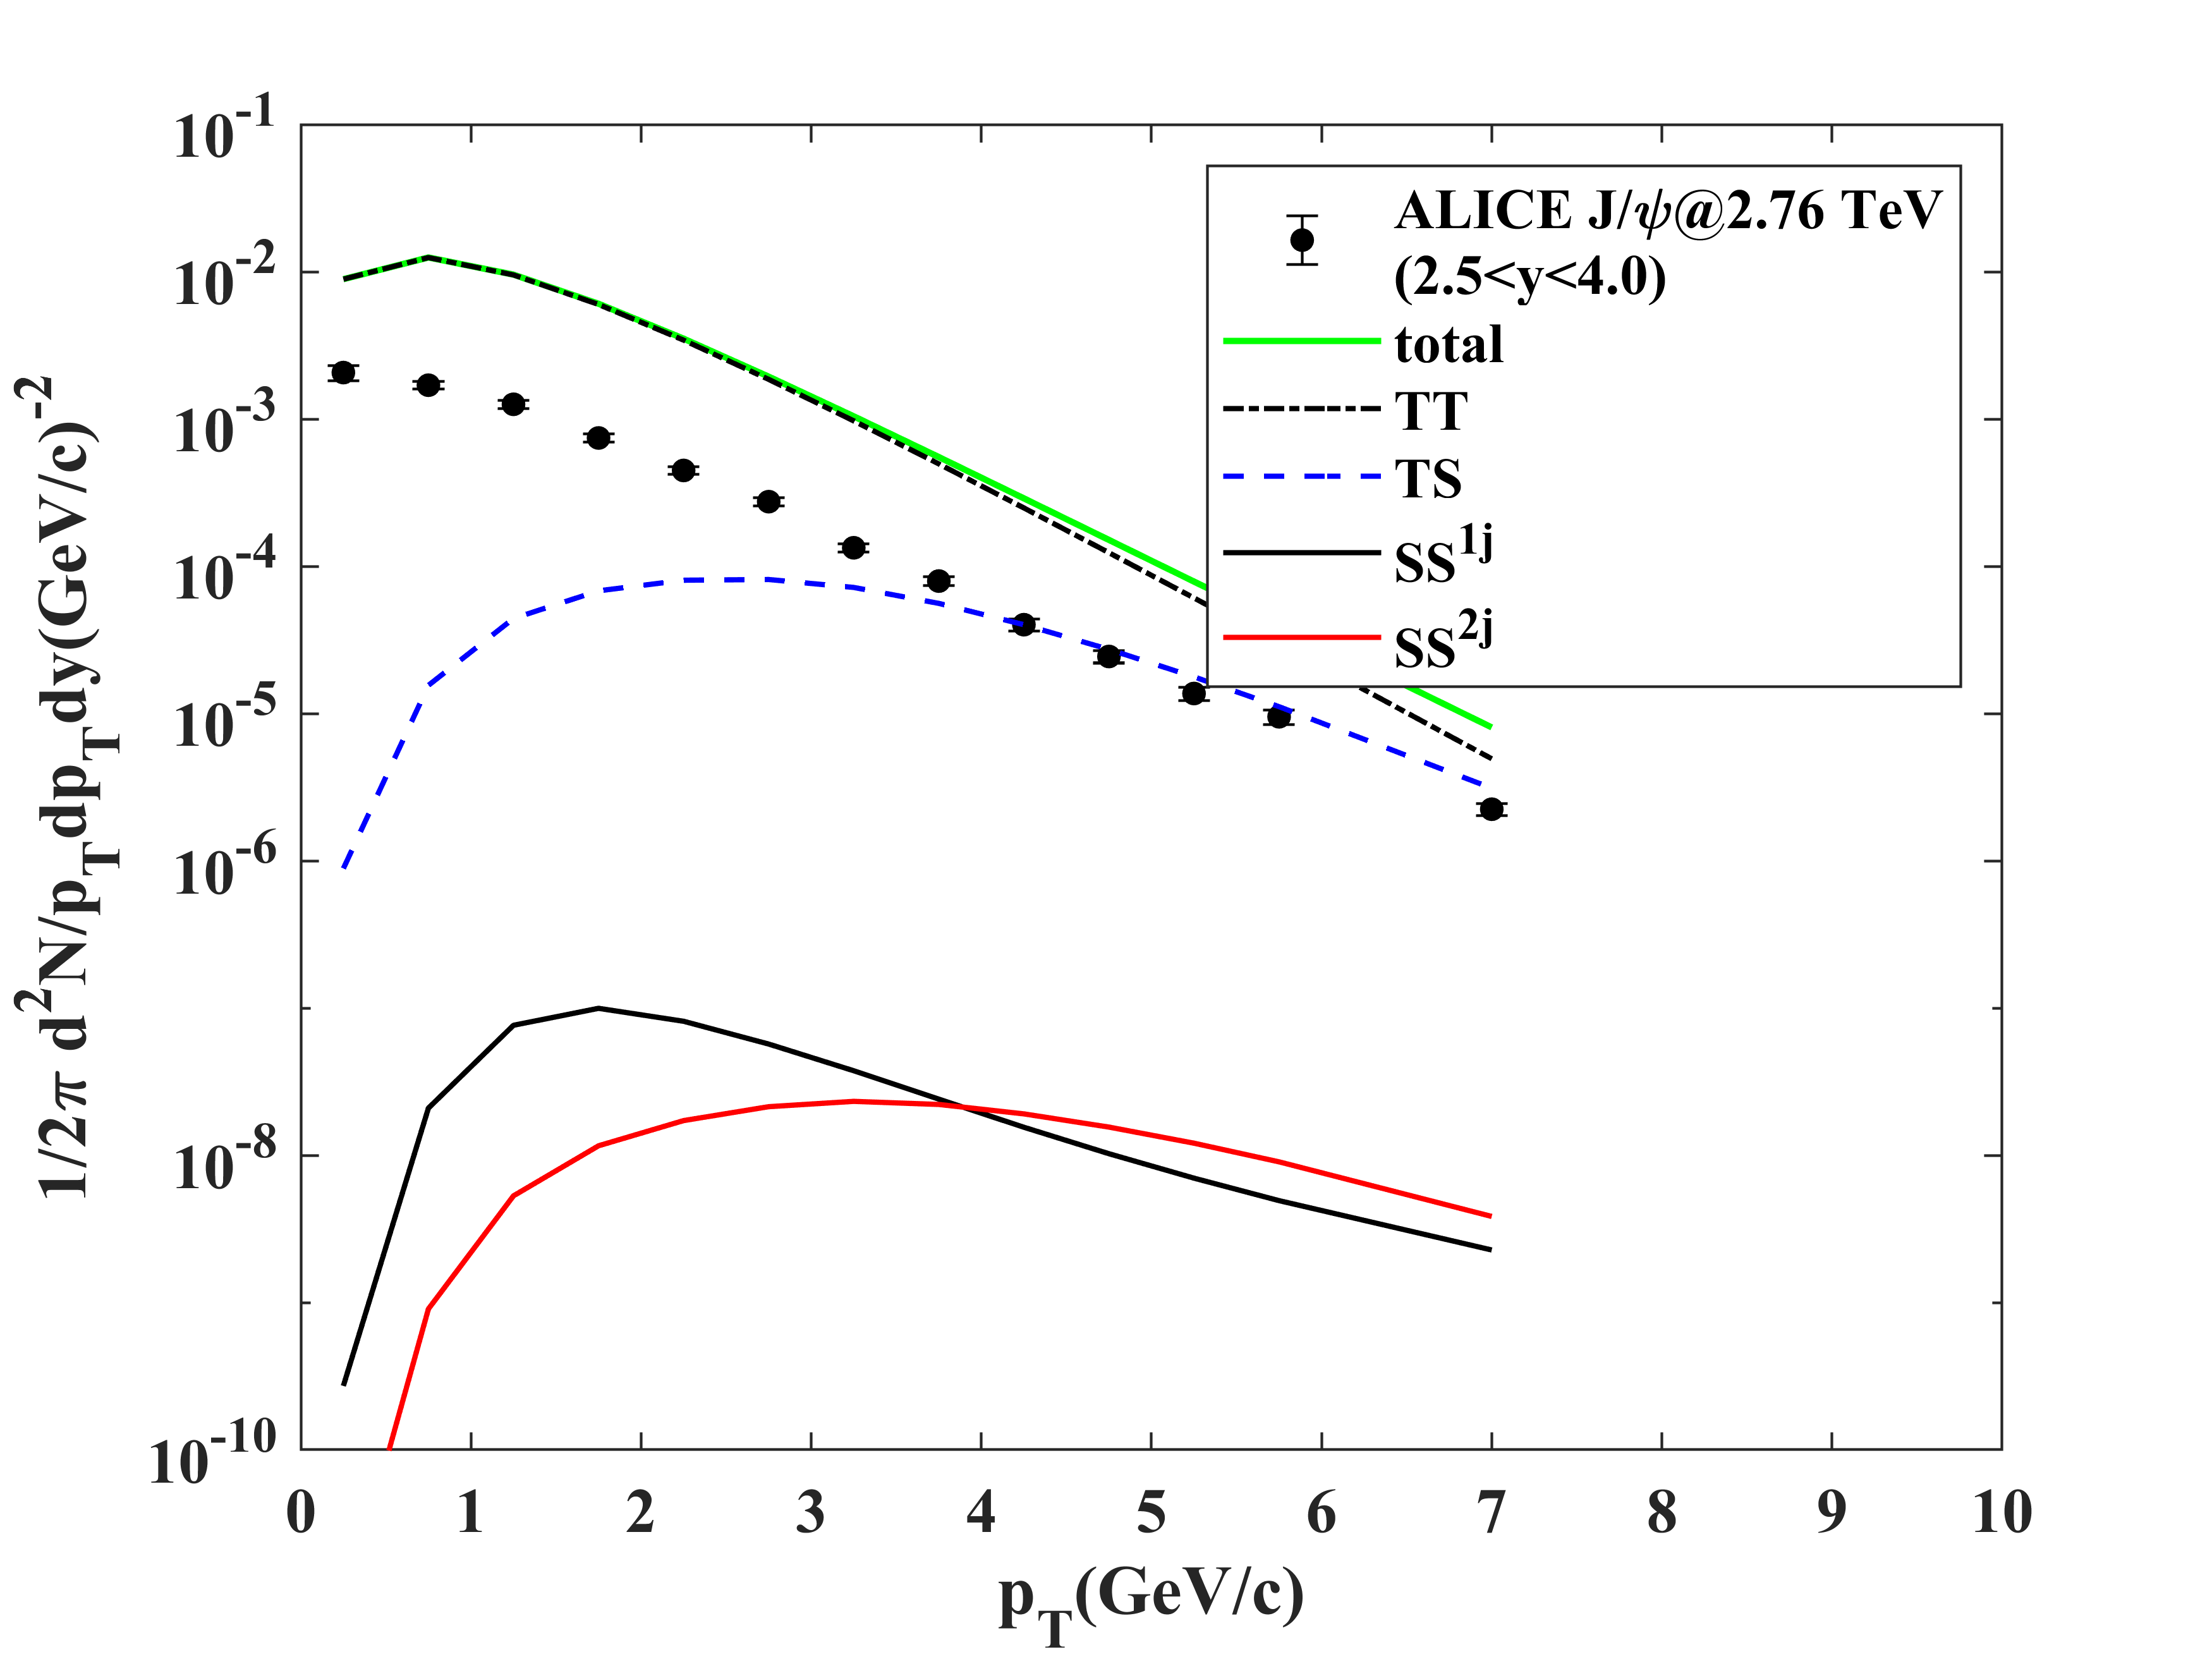
\includegraphics[width=0.9\linewidth]{230704_Jpsi_276.png}
		\caption{2.76 TeV $J/\psi$}
	\end{minipage}
    \begin{minipage}{0.3\linewidth}
    	\centering
    	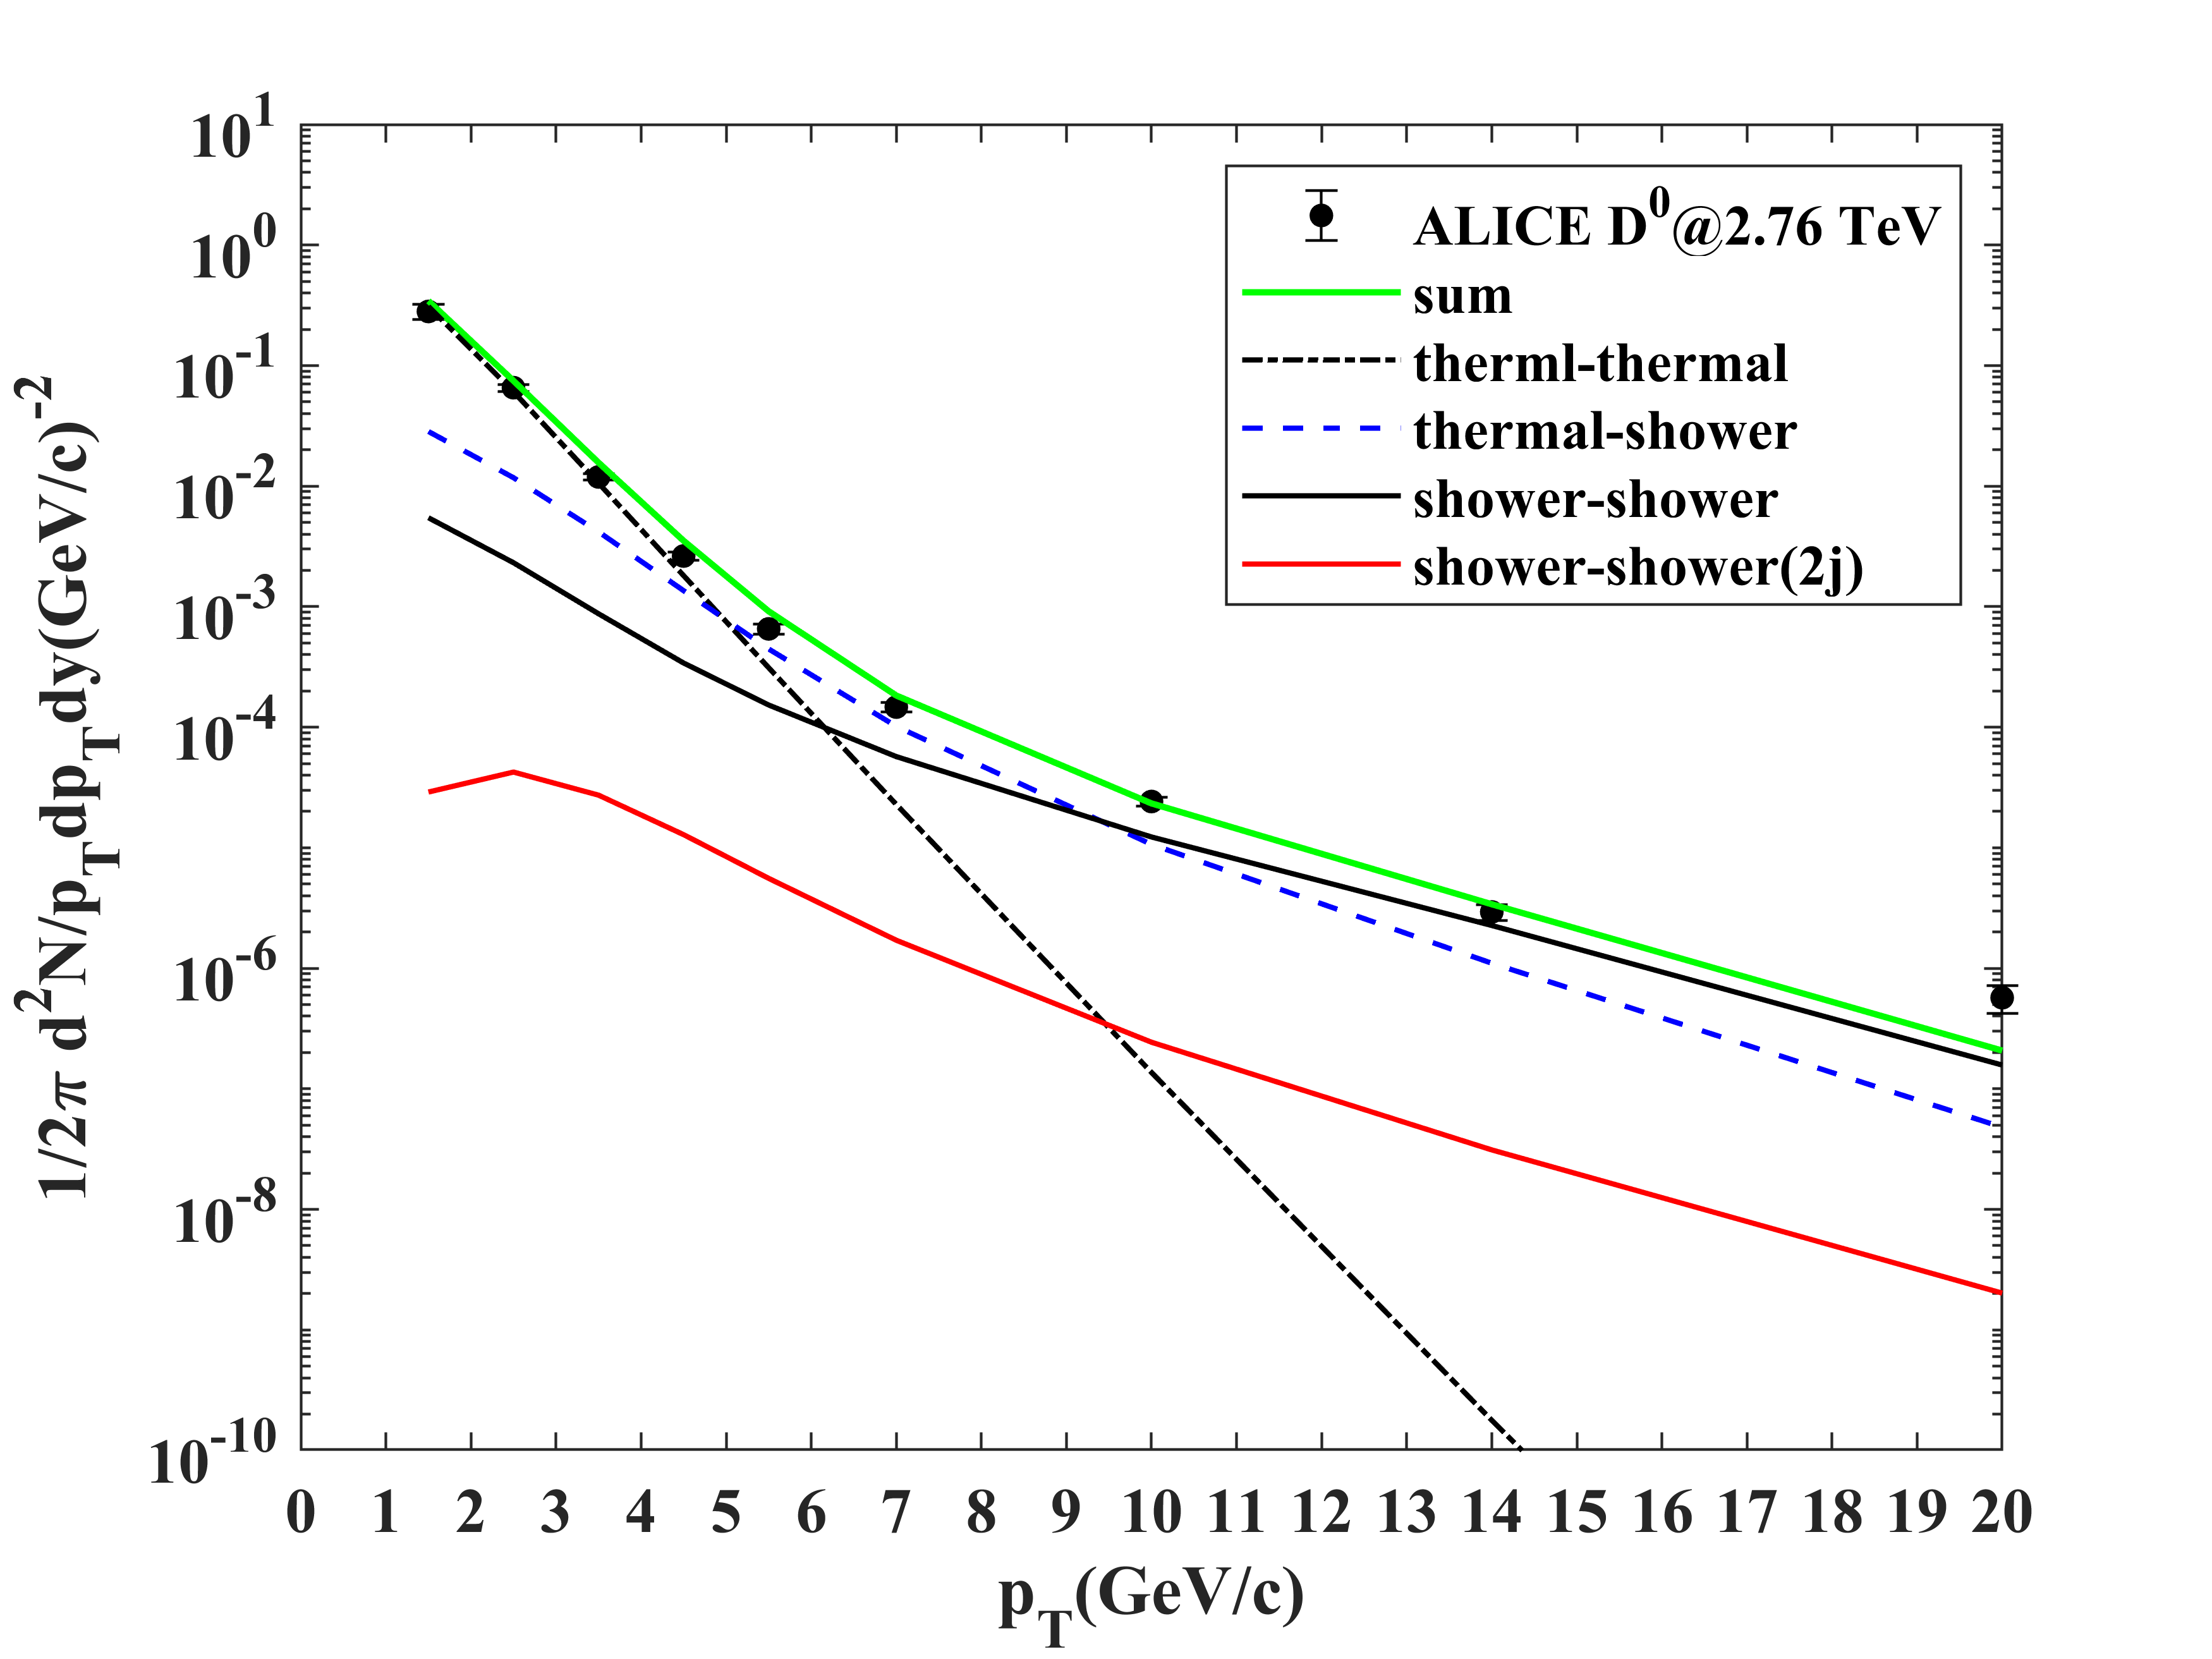
\includegraphics[width=0.9\linewidth]{230704_D0_276.png}
    	\caption{2.76 TeV $D^0$}
    \end{minipage}
	\begin{minipage}{0.3\linewidth}
		\centering
		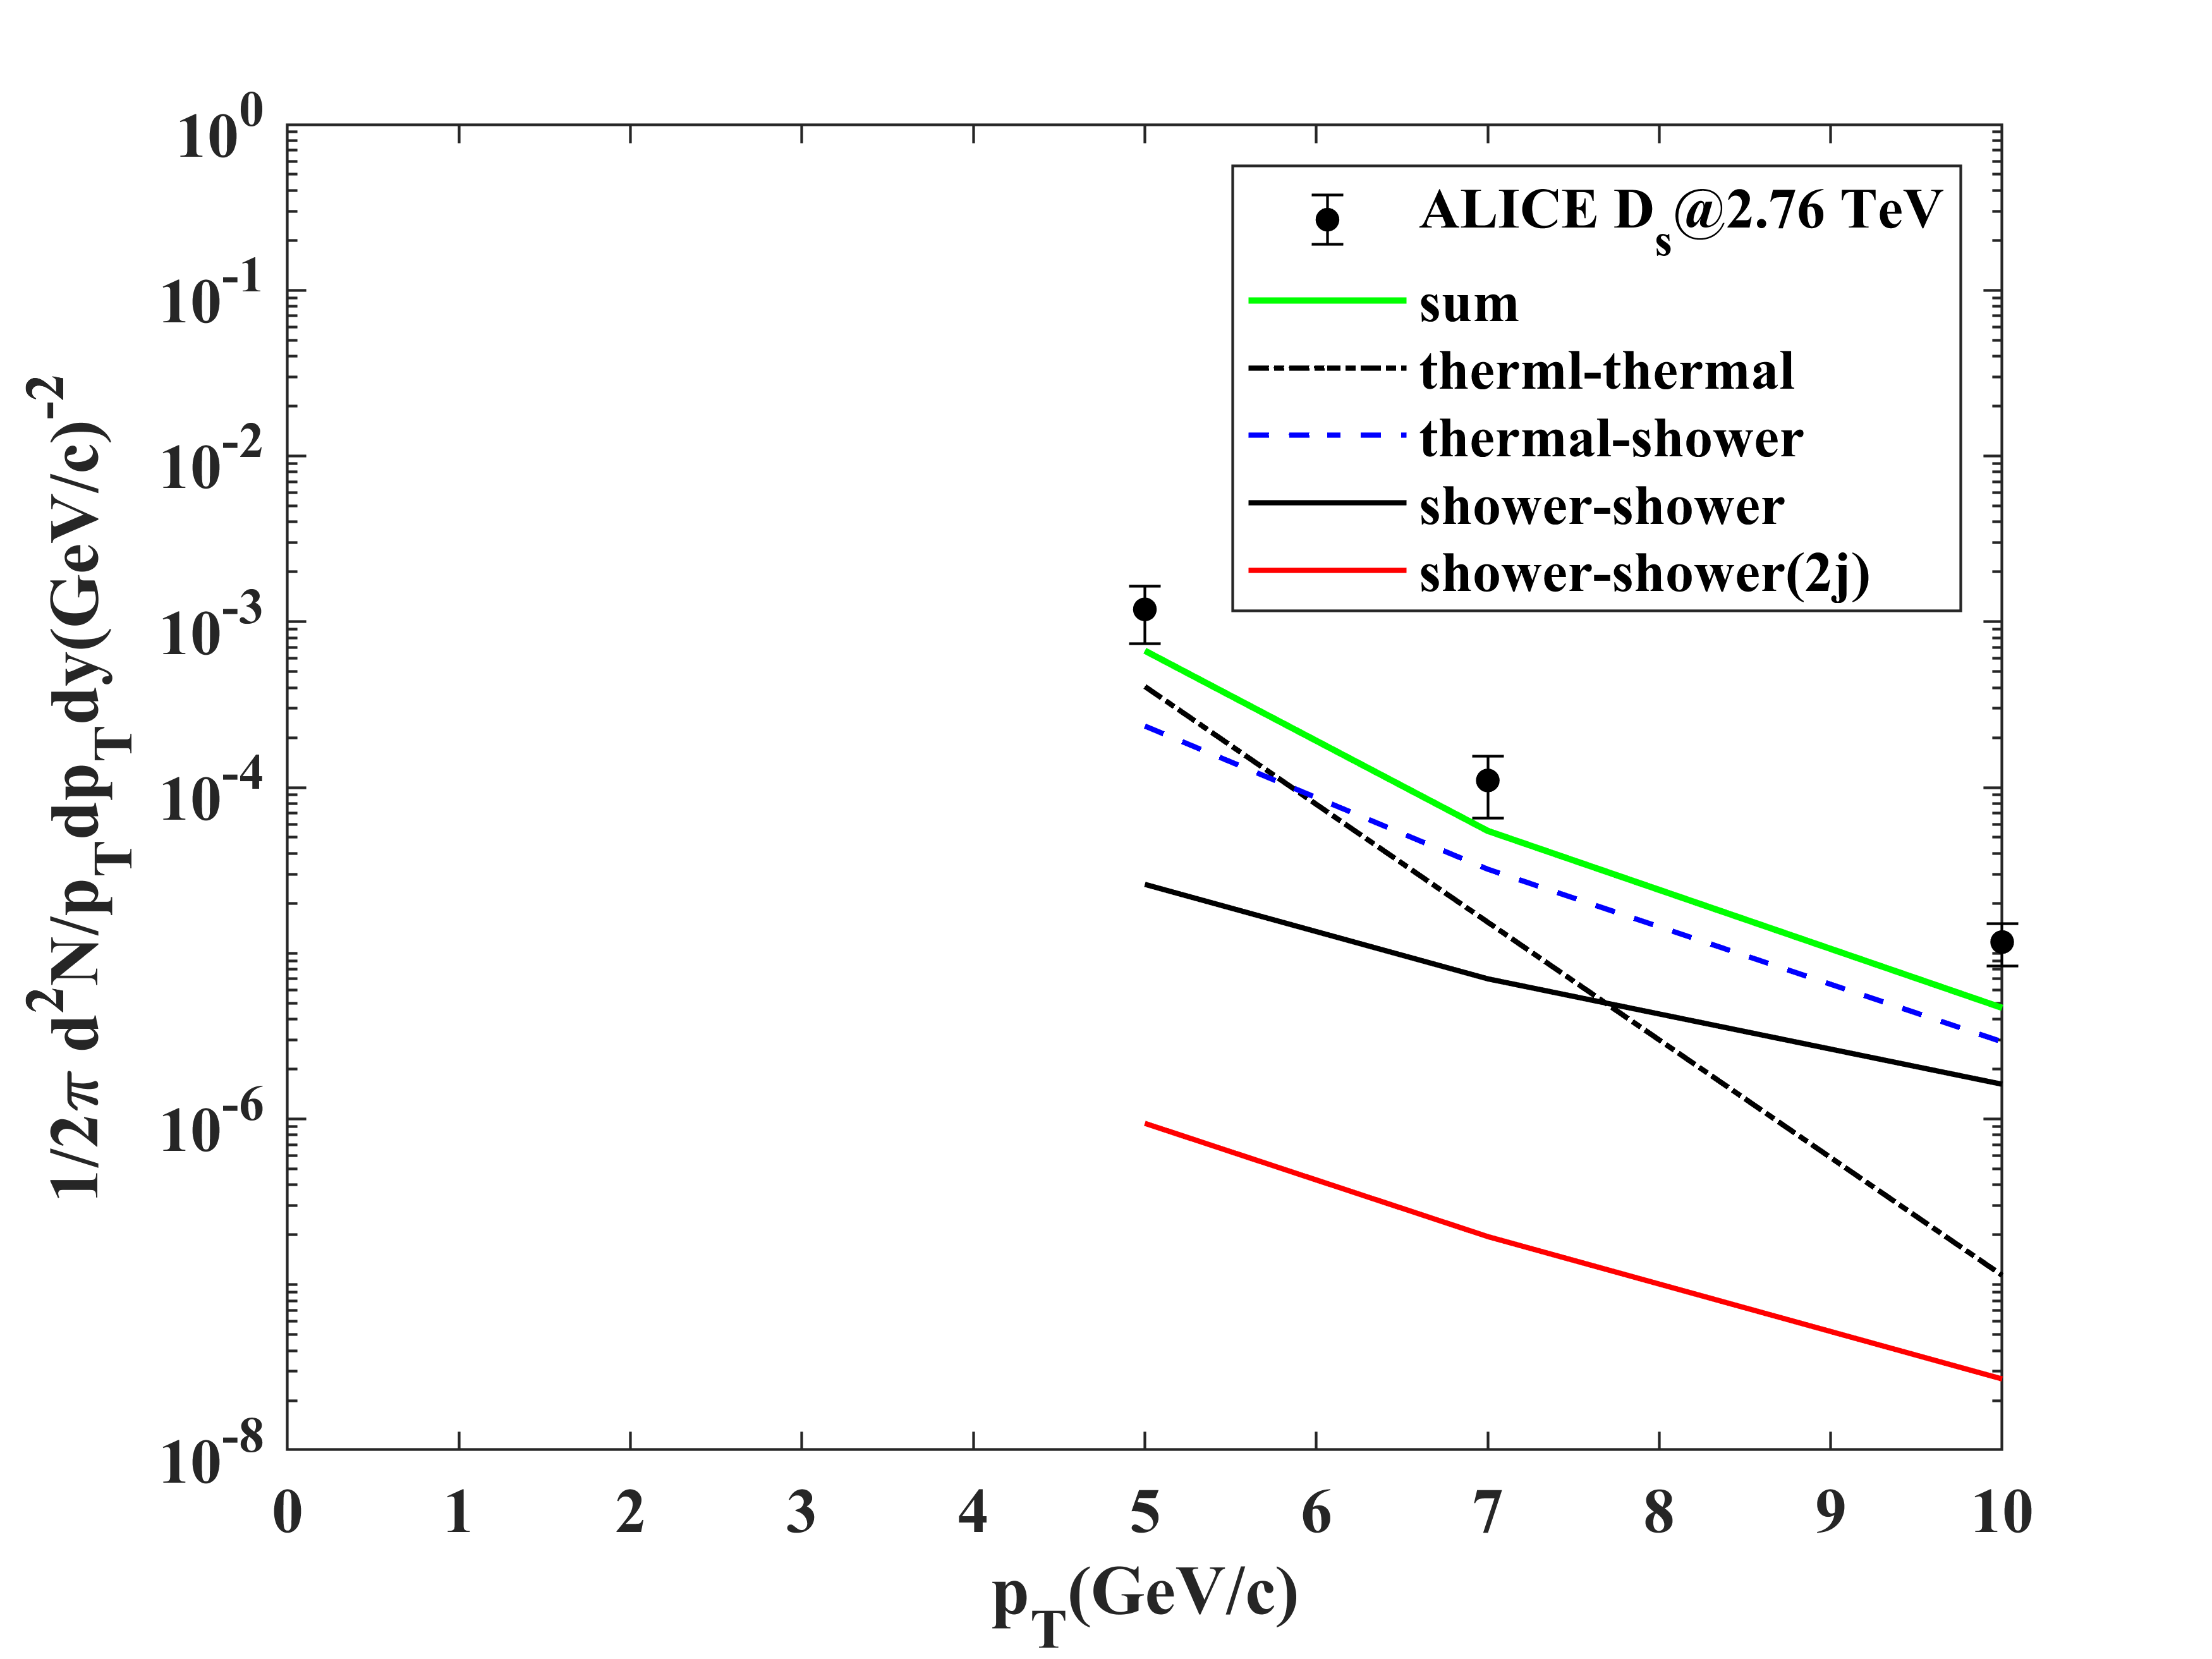
\includegraphics[width=0.9\linewidth]{230704_Ds_276.png}
		\caption{2.76 TeV $D_s$}
	\end{minipage}
	
	\qquad
	
	\begin{minipage}{0.3\linewidth}
		\centering
		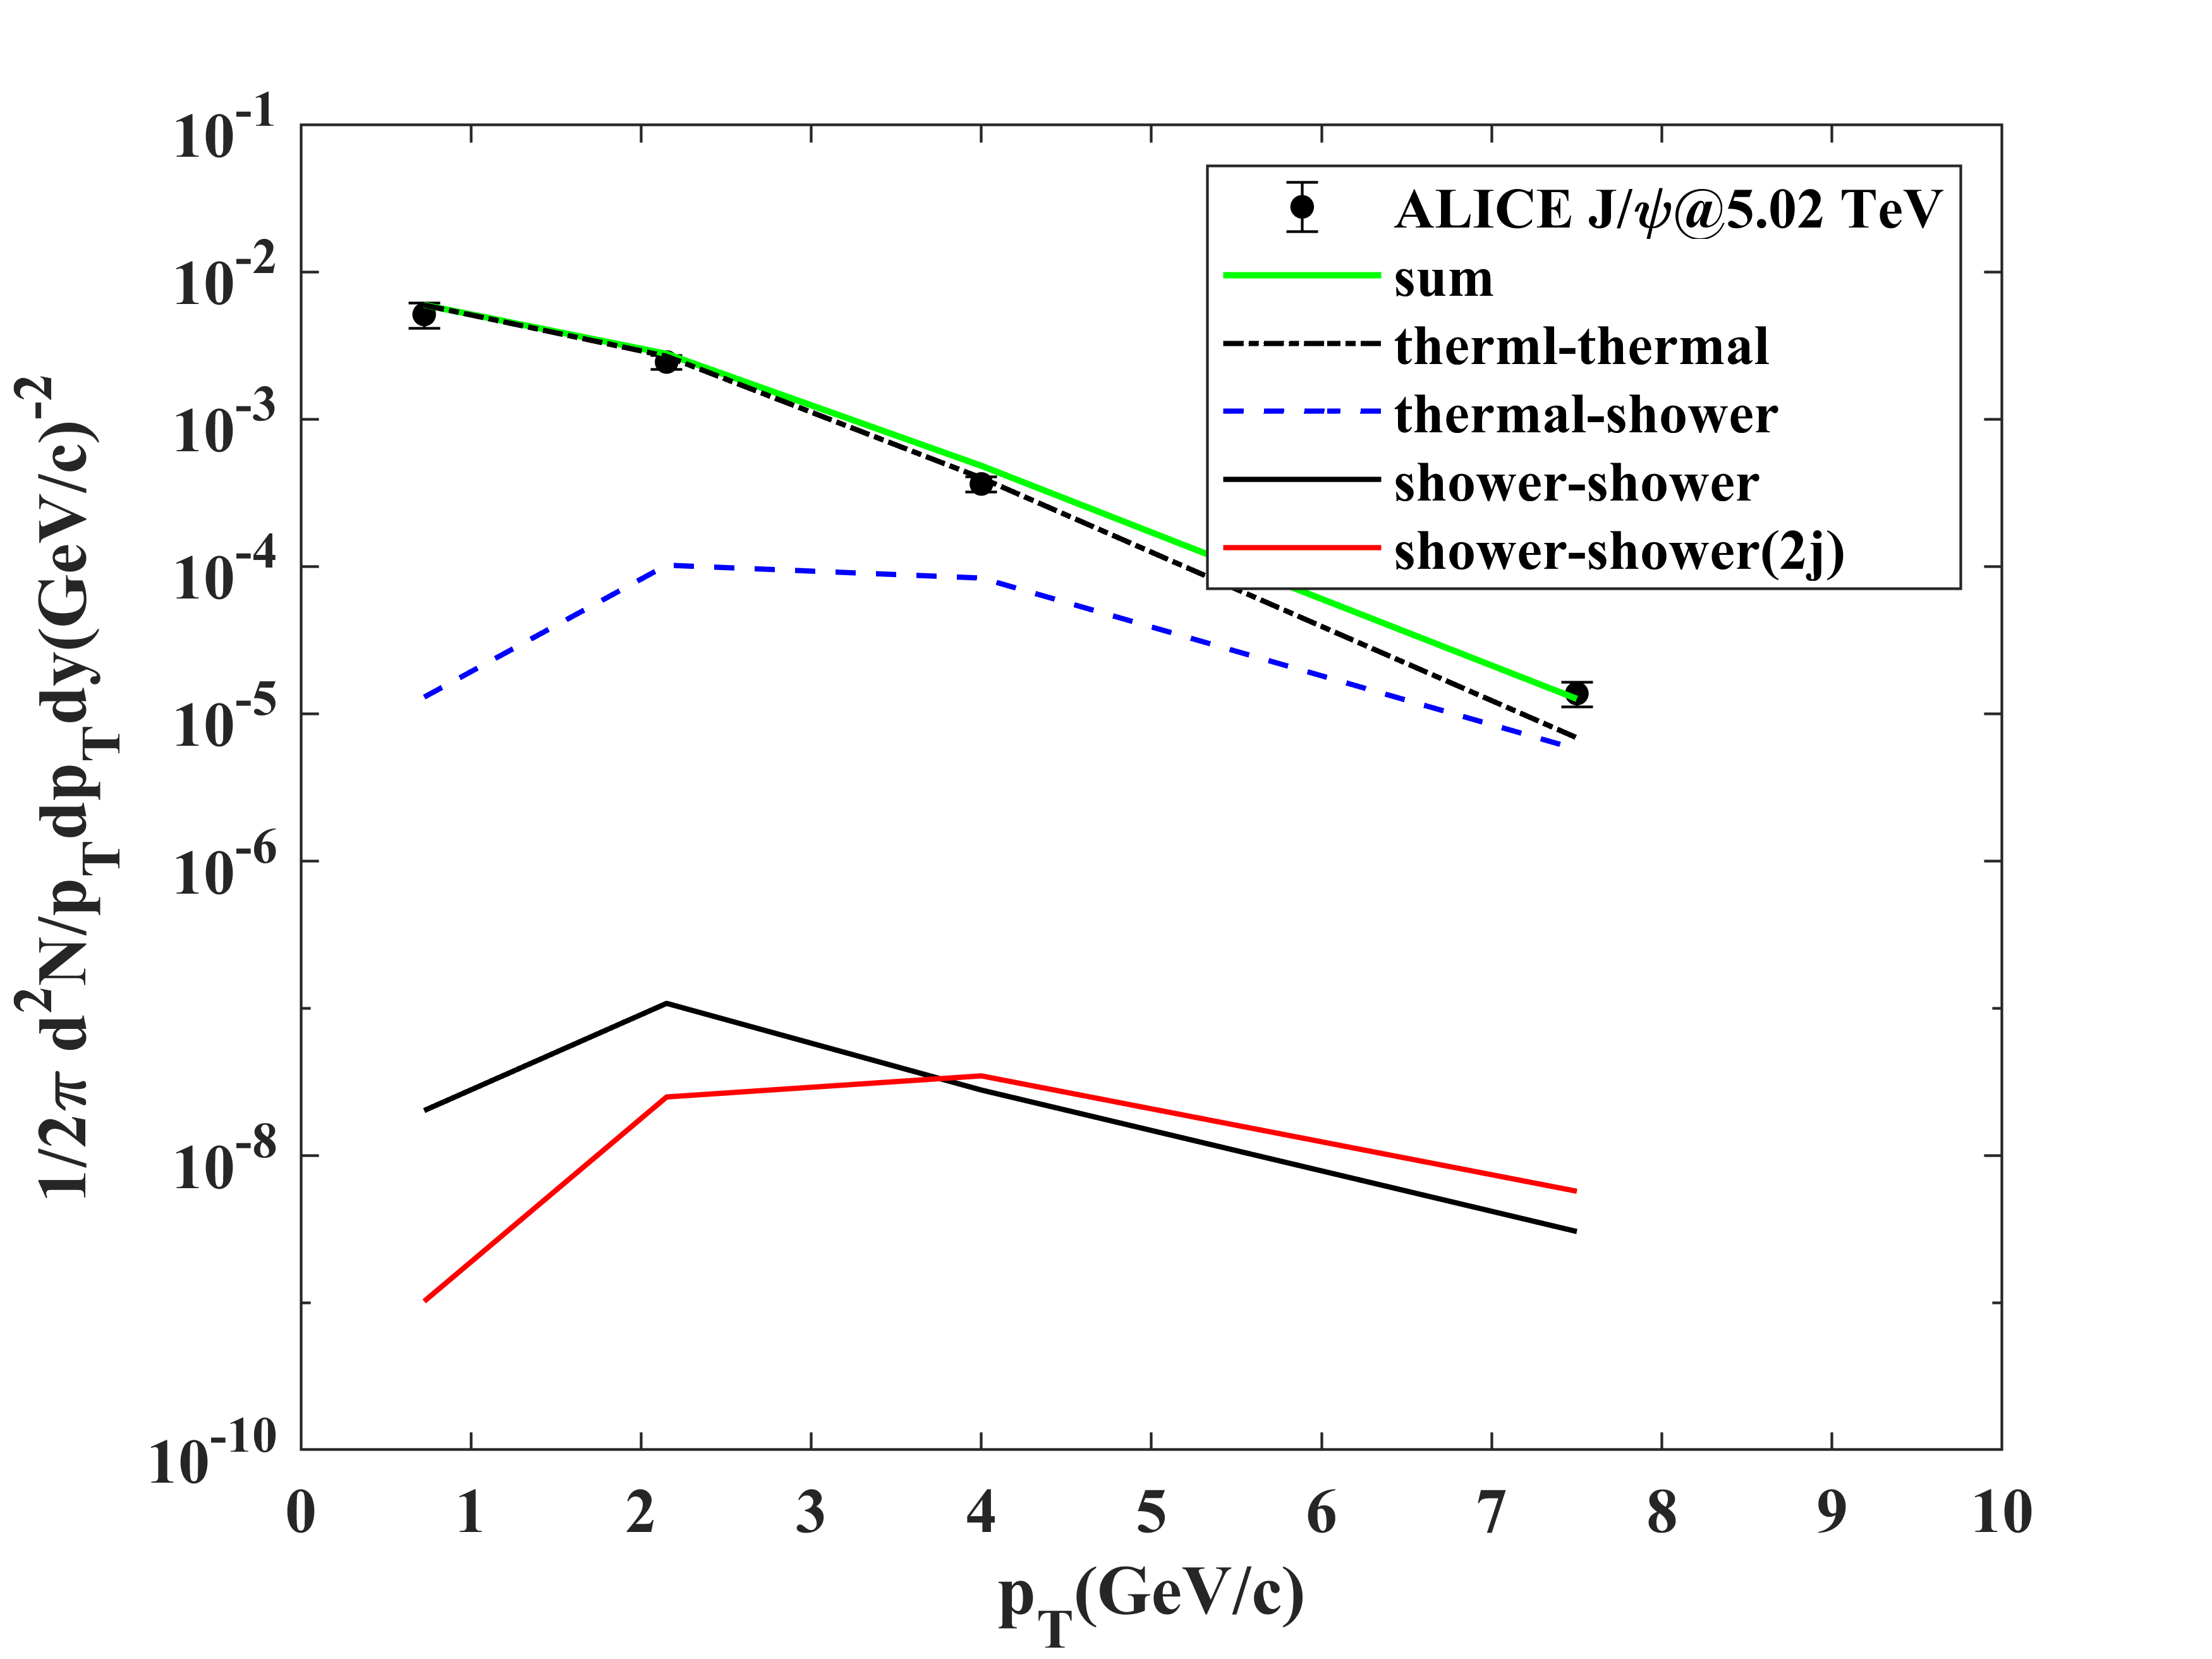
\includegraphics[width=0.9\linewidth]{230704_Jpsi_502.png}
		\caption{5.02 TeV $J/\psi$}
	\end{minipage}
	\begin{minipage}{0.3\linewidth}
		\centering
		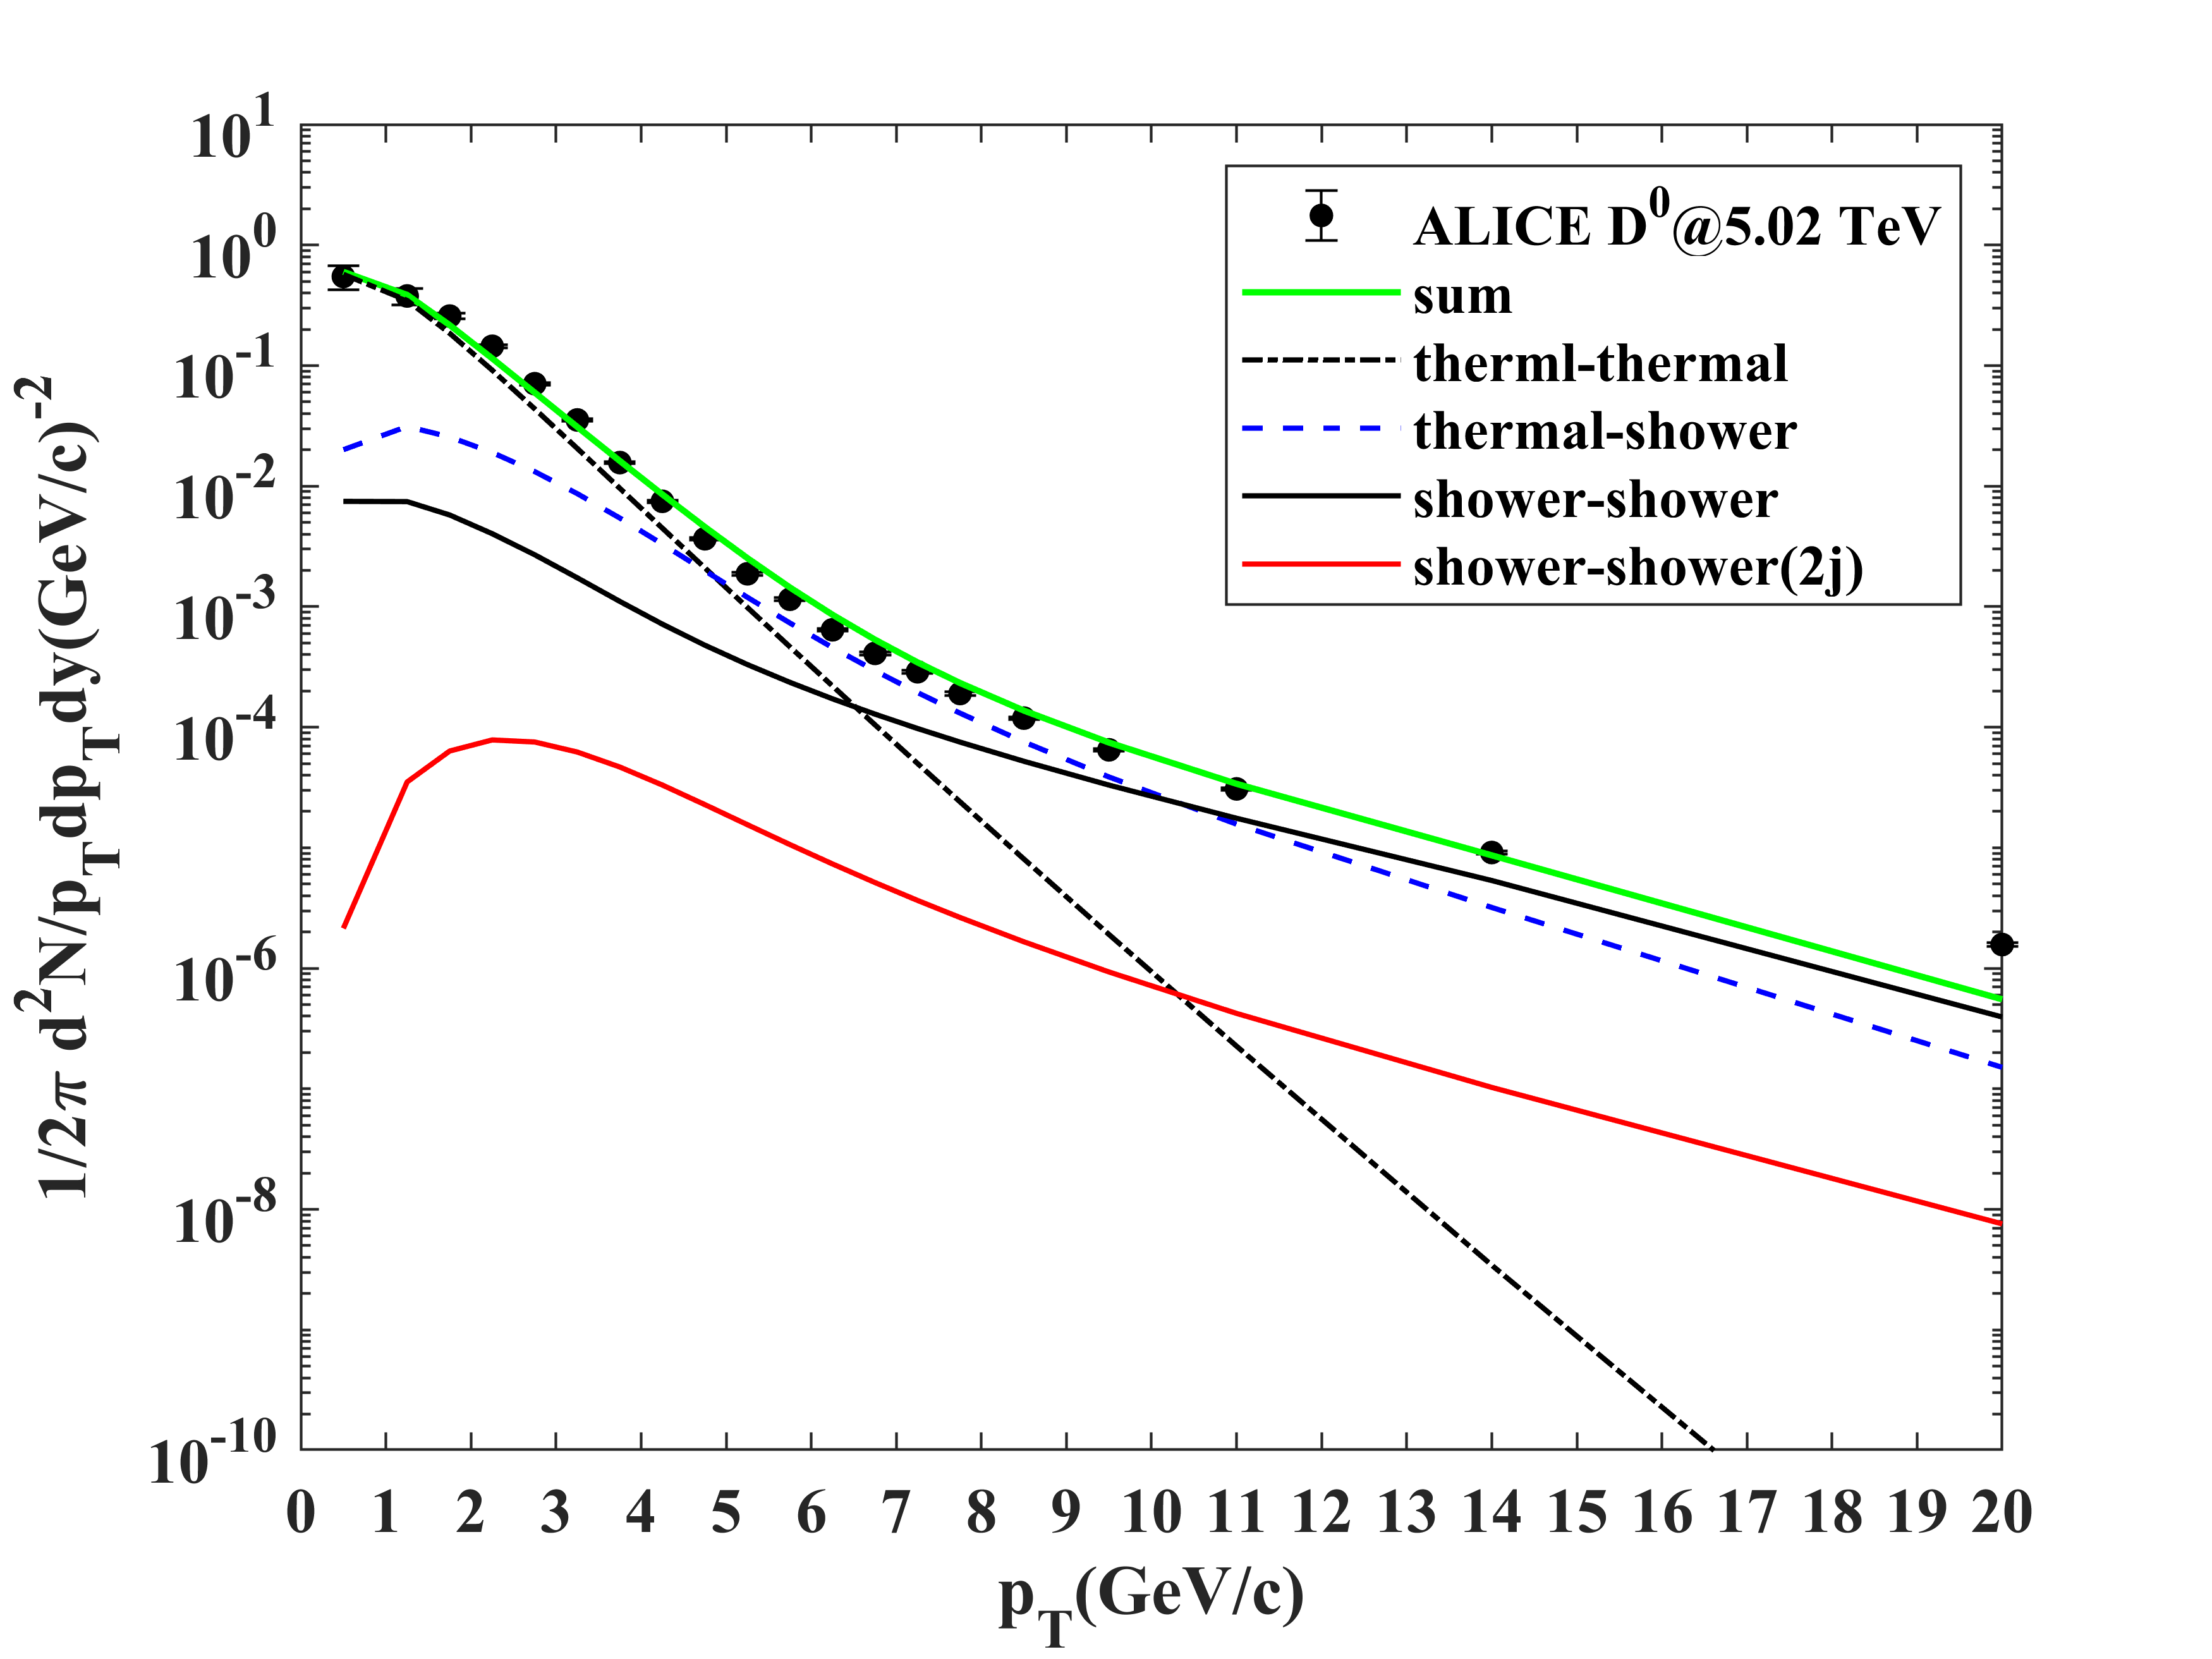
\includegraphics[width=0.9\linewidth]{230704_D0_502.png}
		\caption{5.02 TeV $D^0$}
	\end{minipage}
	\begin{minipage}{0.3\linewidth}
		\centering
		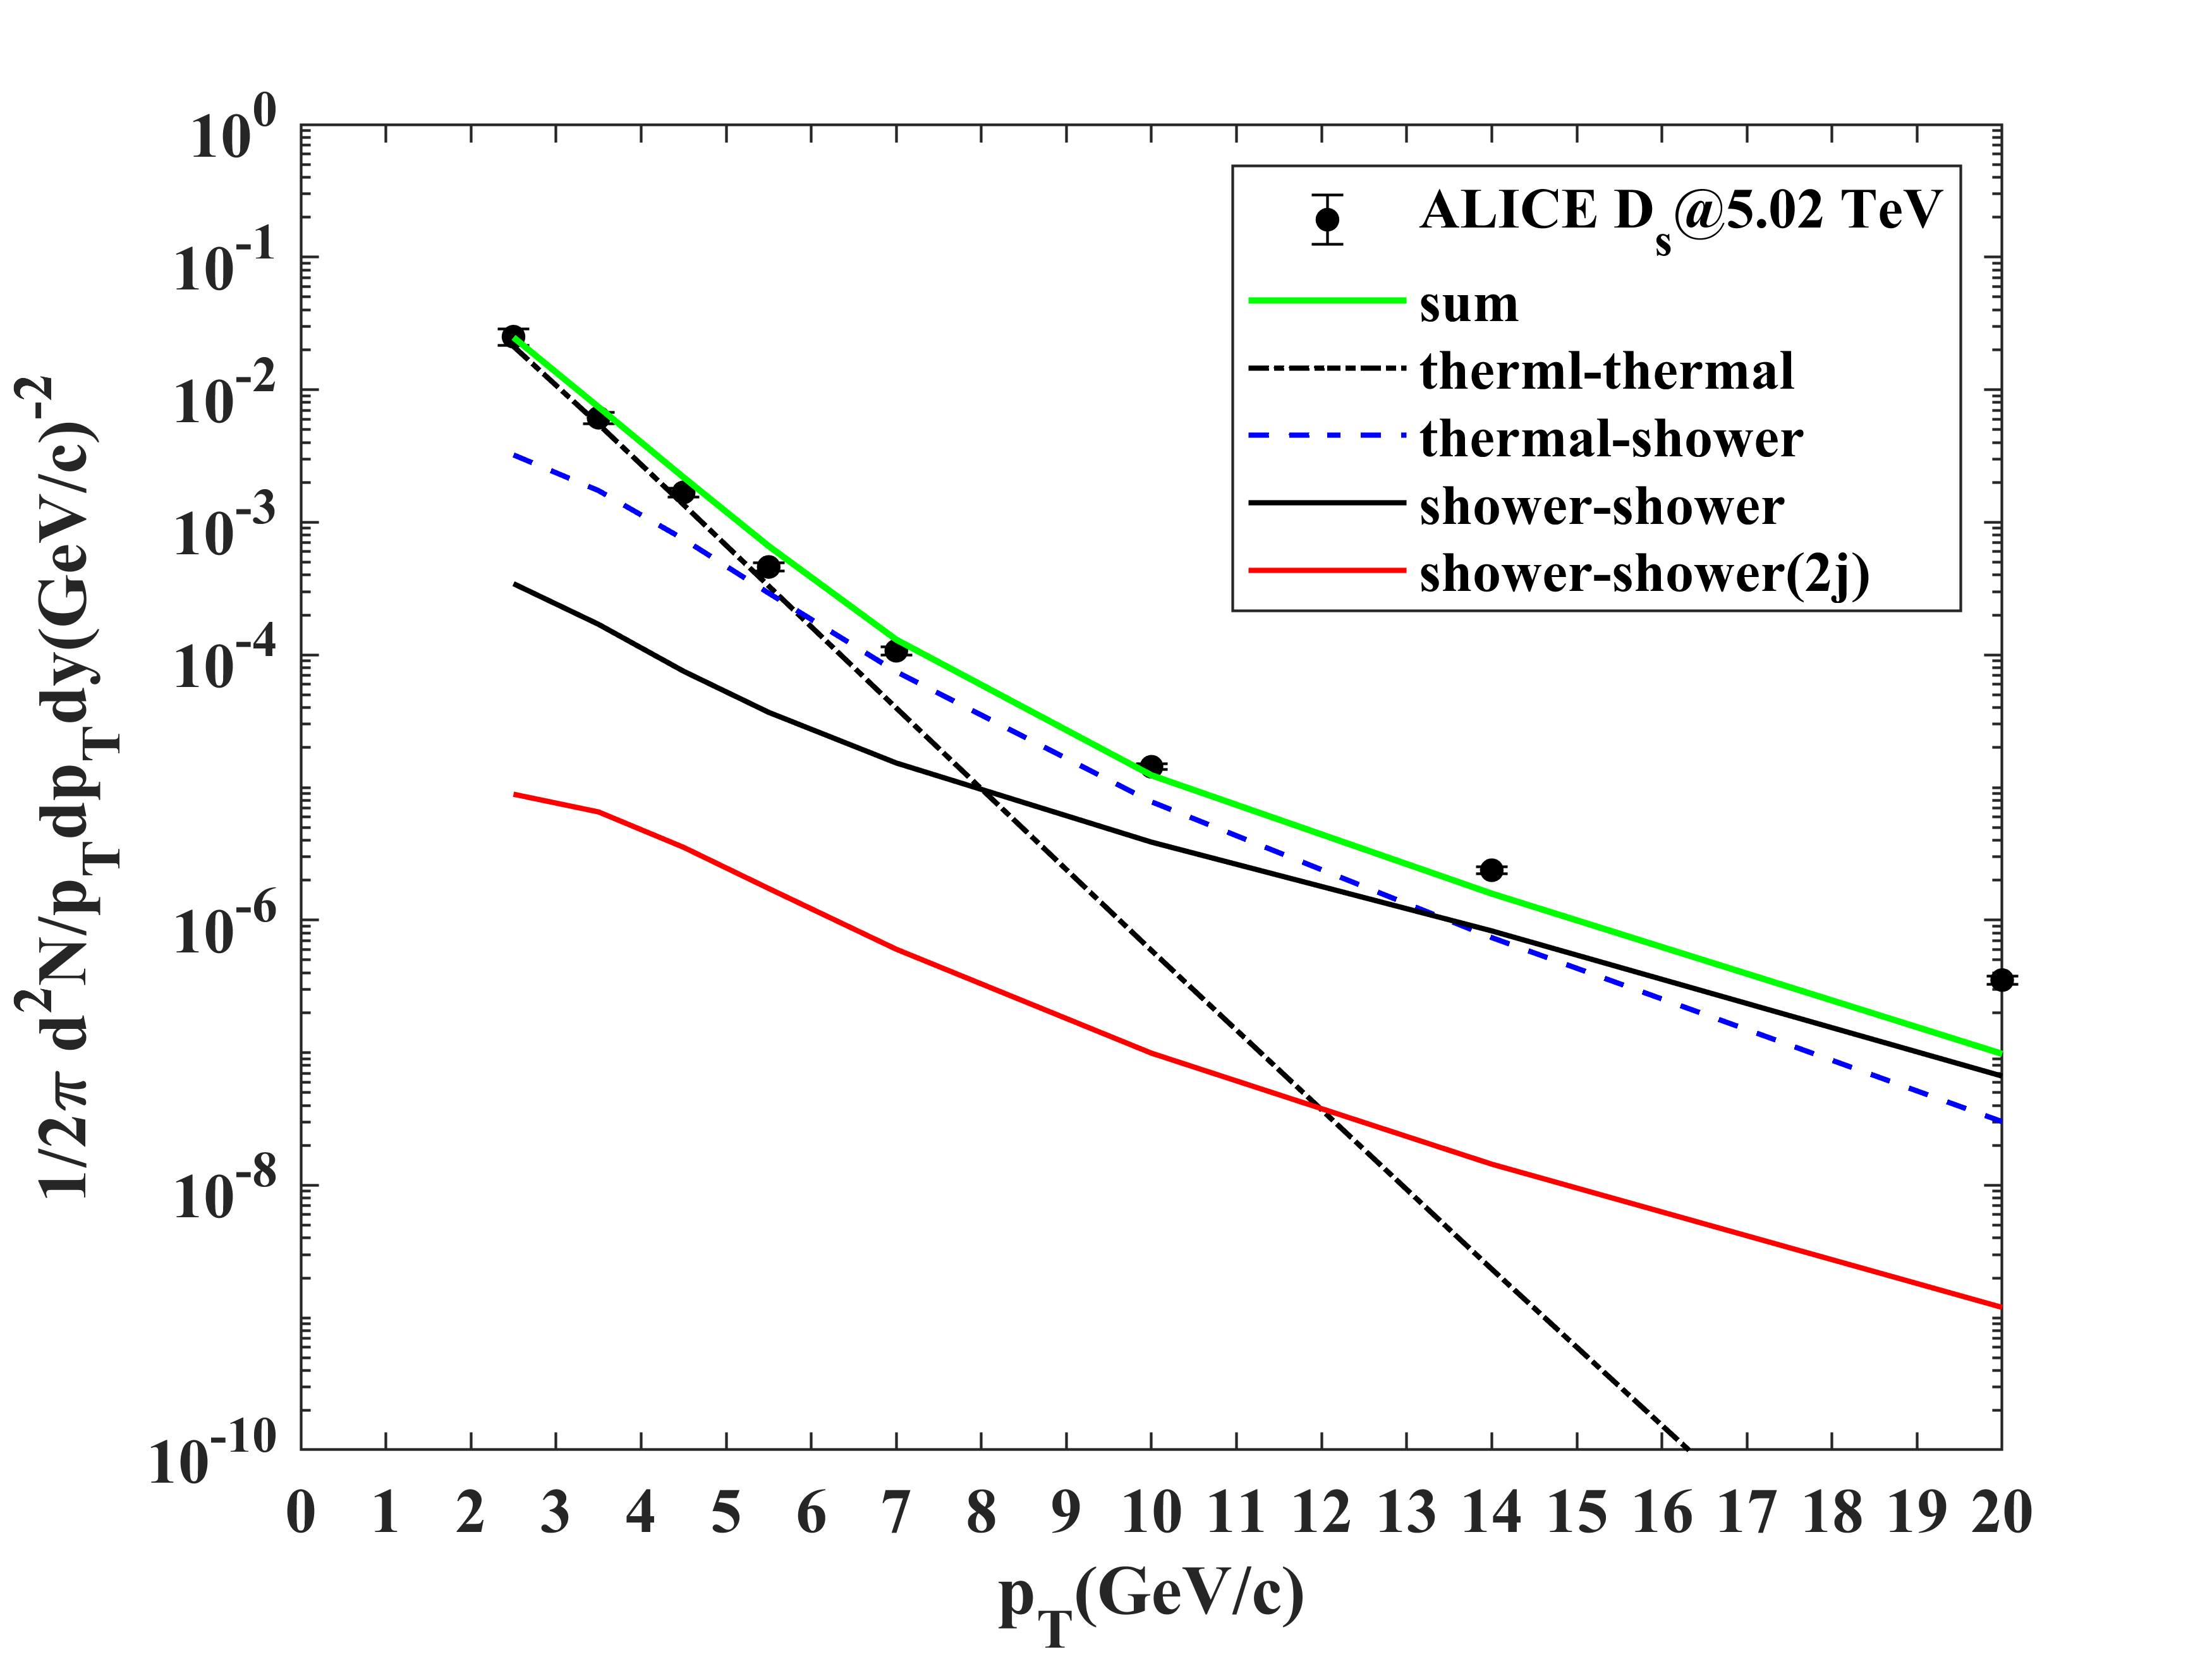
\includegraphics[width=0.9\linewidth]{230704_Ds_502.png}
		\caption{5.02 TeV $D_s$}
	\end{minipage}
	
	\caption{Results of parameters in Tab.\ref{parameters0704}.}
\end{figure}

	
	
	\begin{thebibliography}{99}

		
		
	\end{thebibliography}
	
\end{document}